\documentclass[
		11pt,
		a4paper,
		toc=listof, %% Abbildungs- und Tabellenverzeichnis mit ins Inhaltsverzeichnis
		bibliography=totoc %% Quellenverzeichnis mit ins Inhaltsverzeichnis
		]{scrreprt}	 %% KOMA Script

% HTWG
\usepackage{graphicx}
\usepackage{a4}
\usepackage{german}

% Eigene
\usepackage[utf8]{inputenc} %% Umlaute
\usepackage[dua]{acronym} %% Abkuerzungsverzeichnis (nur verwendete)
\usepackage{todonotes} %% TODOs moeglich mit \todo{}
\usepackage{booktabs} %% Tabellen
\usepackage{amsmath} %% Formeln
\usepackage{listings} %% Codebeispiele
\usepackage{subfigure} %% Mehrere Bilder nebeneinander
\PassOptionsToPackage{hyphens}{url}\usepackage{hyperref} %% referenzen innerhalb und außerhalb des Dokumentes
\usepackage[headsepline]{scrpage2} %%Numerrierung der Seiten + Kapitelnamen in Kopfzeile inkl. Trennstrich
\pagestyle{scrheadings} %% die folgenden Zeilen sorgen für die korrekte Nummerierung und deren Anzeige 
\clearscrheadfoot %% und für die Kopfzeile mit aktuellem Kapitel etc.
\ihead{\headmark}
\cfoot[\pagemark]{\pagemark}
\automark{chapter}
\usepackage{float} %% Floatpackage um Grafik-Positionen zu forcieren
\newcommand*{\quelle}[1]{\footnotesize Quelle:~#1}

% Eigenes Design 
%TODO loeschen wenn default HTWG Design (was es nicht wirklich gibt) gewuuenscht ist
\usepackage[bottom=3cm]{geometry}
\usepackage{setspace}
\onehalfspacing


% KOMA script anpassungen 
%TODO entfernen wenn kein KOMA Script gewuenscht
\usepackage{scrhack}

%%%%%%%% Codebeispiele
\usepackage{color}
\usepackage{xcolor}
\usepackage{listings}
\usepackage{caption}

\setcounter{tocdepth}{2}  %% Uebreschriften bis subsectionw ins Inhaltsverzeichnis
\setcounter{secnumdepth}{3}  %% Nummerierung bis subsection


%%% Codebeispiele - Style
\DeclareCaptionFont{white}{\color{white}}
\DeclareCaptionFormat{listing}{\colorbox{gray}{\parbox{\textwidth}{#1#2#3}}}
\captionsetup[lstlisting]{format=listing,labelfont=white,textfont=white}

% Entfernt Kapitel Ueberschrift
% Bsp.
% 	ALT:
%       Kapitel 1
%       Einführung
%
% 	NEU:
% 		1 Einführung
%
\renewcommand*\chapterheadstartvskip{\vspace{-\topskip}}
\newcommand{\thema}{Dokumentation Teamprojekt}
\newcommand{\forschungsfrage}{Autonomes Fahren in der DuckieTown-Umgebung - Lokalisierung mit einem Deep-Learning Ansatz}
\newcommand{\abgabedatum}{\today}
\newcommand{\firstauthor}{Stephan Perren}
\newcommand{\secondauthor}{Felix Mayer}
\newcommand{\studiengang}{Angewandte Informatik}
\newcommand{\betreuer}{Prof. Dr. Oliver Bittel}

\setlength\parindent{0pt}

\lstset{
	frame=top,frame=bottom,
	basicstyle=\small\normalfont\sffamily,    % the size of the fonts that are used for the code
	stepnumber=1,                           % the step between two line-numbers. If it is 1 each line will be numbered
	numbersep=2pt,                         % how far the line-numbers are from the code
	tabsize=1,                              % tab size in blank spaces
	extendedchars=true,                     %
	breaklines=true,                        % sets automatic line breaking
	captionpos=t,                           % sets the caption-position to top
	mathescape=true,
	stringstyle=\color{white}\ttfamily, % Farbe der String
	showspaces=false,
	showtabs=false,            
	xleftmargin=17pt,
	framexleftmargin=17pt,
	framexrightmargin=17pt,
	framexbottommargin=5pt,
	framextopmargin=5pt,
	showstringspaces=false,
	numbers=left
}

\DeclareCaptionFormat{listing}{\rule{\dimexpr\textwidth+17pt\relax}{0.4pt}\par\vskip1pt#1#2#3}
\captionsetup[lstlisting]{format=listing,singlelinecheck=false, margin=0pt, font={sf},labelsep=space,labelfont=bf}

\renewcommand{\lstlistingname}{Codebeispiel}

\begin{document}
%% Nummerierung aus
\pagenumbering{gobble}

% HTWG Templates fuer Titelseite etc.

\begin{titlepage}

\vspace*{-3.5cm}

\begin{center}

\includegraphics[width=5cm]{htwg/htwg-logo}

Fakultät Informatik \\
Fachbereich Wirtschaftsinformatik
\end{center}

\vspace*{1.5cm}

\begin{center}
	\huge{
		\textbf{\thema} \\[1cm]
	}
	\normalsize{
		\textbf{\forschungsfrage} \\[2cm]
	}
\end{center}
\begin{tabular}{p{6cm}p{5cm}}
                 \bfseries{Name:} & \autor \\\\
                 \bfseries{Arbeitsplatz:} & \firma  \\\\
                 \bfseries{Erstkorrektor:} & \erstbetreuer \\\\
                 \bfseries{Zweitkorrektor:} & \zweitbetreuer \\\\
                 \bfseries{Abgabetermin:} & \abgabedatum \\\\
\end{tabular}
\\[1cm]
\begin{flushright}
	Konstanz, \abgabedatum \\[0.5cm]
	Der Vorsitzende des Prüfungsausschusses \\[1.5cm]
	Prof. Dr. Wilhelm Erben
\end{flushright}
\end{titlepage}
\pagenumbering{Roman}
\tableofcontents
\addcontentsline{toc}{chapter}{Inhaltsverzeichnis}
\addchap{Abkürzungsverzeichnis}

\begin{acronym}[ROS]
	\acro{mit}[MIT]{Massachusetts Institute of Technology}
	\acro{ain}[AIN]{Angewandte Informatik}
	\acro{ros}[ROS]{Robot Operating System}
\end{acronym}


\clearpage
%% Starte Paginierung
\pagenumbering{arabic}

\chapter{Einleitung}

\begin{figure}[H]
	\centering
	\begin{minipage}{.5\textwidth}
		\centering
		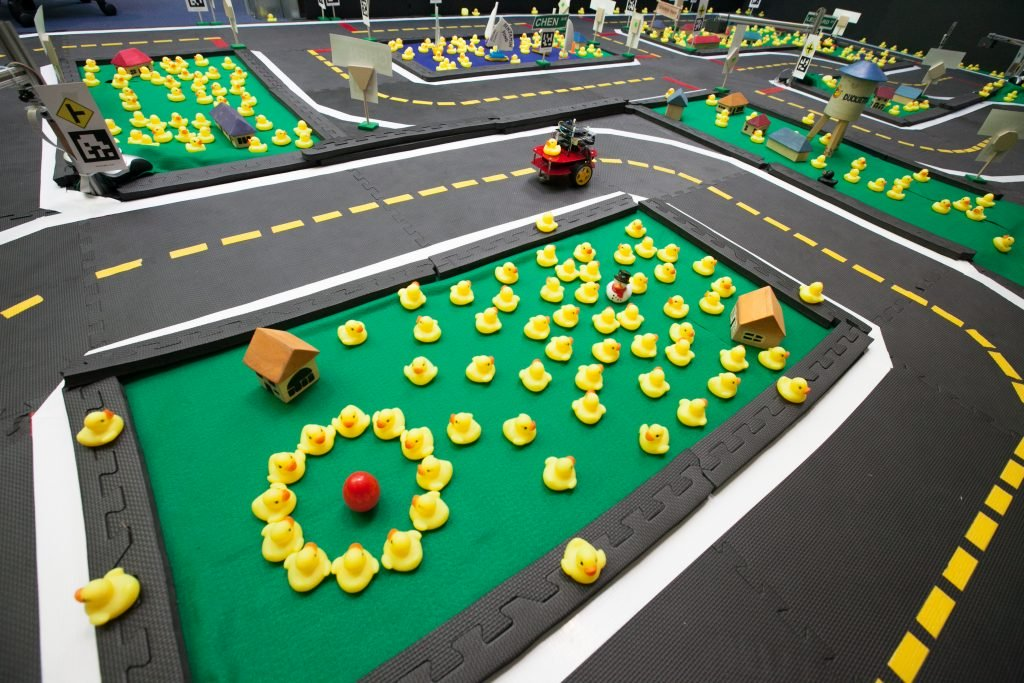
\includegraphics[width=0.95\textwidth]{kapitel1/images/duckietown.png}
		\quelle\url{https://www.duckietown.org/wp-content/uploads/2018/05/duckietown_nice-1024x683.jpg}
		\label{fig:duckietown}
	\end{minipage}%
	\begin{minipage}{.5\textwidth}
		\centering
		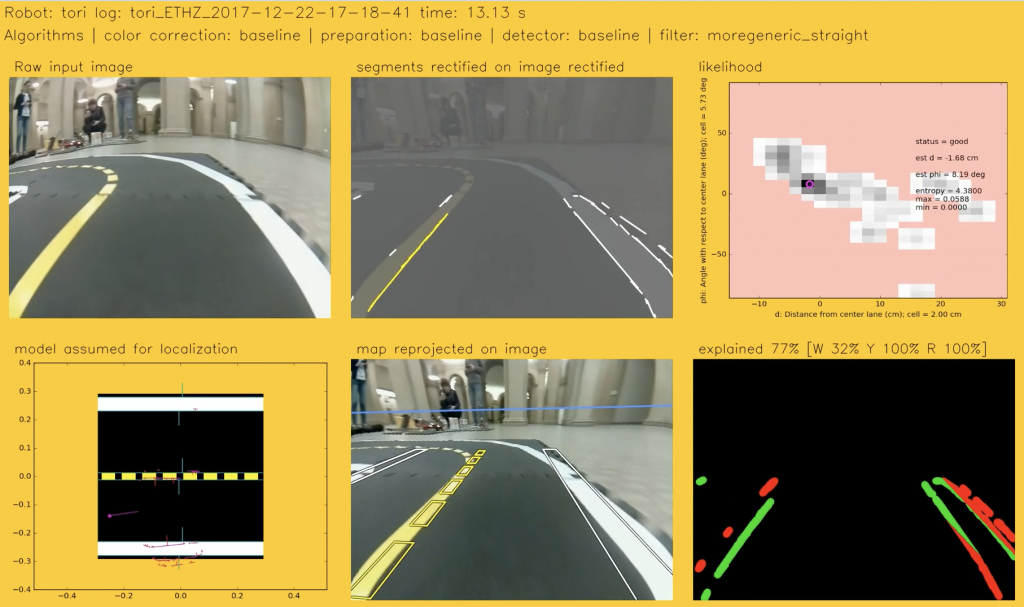
\includegraphics[width=1.072\textwidth]{kapitel1/images/duckietown2.png}
		\quelle\url{https://www.duckietown.org/wp-content/uploads/2018/06/data-from-img-CameraDataProcessed-fc6fd822-1024x607.png}
		\label{fig:duckietown2}
	\end{minipage}
	\caption{Duckietown}
\end{figure}

Das Duckietown-Projekt wurde 2016 am \acf{mit} konzipiert. Das Ziel war es, eine Plattform zu
entwickeln, die klein, kostengünstig und \grqq smart\grqq{} ist, aber dennoch die wissenschaftlichen
Herausforderungen einer echten autonomen Roboterplattform anbietet und die Entwicklung
intelligenter autonomer Fahrfunktionen erlaubt. \cite{duckietown}\\

\noindent Ziel des AIN-Projekts ist die Implementierung verschiedener klassischer Robotik-Algorithmen
für Navigation und Lokalisierung mit dem Duckietown-Simulator\\

\noindent Nach einer Einarbeitung in die Fähigkeiten des Simulators sollen Algorithmen für die
Linienverfolgung, Lokalisierung mit einem Partikelfilter bei bekannter Umgebungskarte,
Navigation (Planung, Wegeverfolgung und Hindernisvermeidung) realisiert werden. Ein Multi-
Vehicle-Szenario soll berücksichtigt werden. Optional können auch KI-Komponenten für
Fahrverhalten und Erkennung von Verkehrszeichen entwickelt werden. Hierzu sollen neue
Techniken wie Deep Neural Networks und Deep Reinforcement Learning zum Einsatz
kommen.\\

\noindent Das Projekt, das für etwa 2-4 Personen vorgesehen ist, soll in Python realisiert werden.
Eventuell kommt \acf{ros} zum Einsatz.

\chapter{DuckieTown}

\section{Umgebung}

In einer DuckieTown-Umgebung wird die Umwelt für einen DuckieBot definiert. Ein DuckieBot kann diese Umgebung dann observieren und sich in dieser bewegen. Eine DuckieTown-Umgebug wird dabei aus verschiedenen Kacheln und Objekten aufgebaut. Bei den Kacheln wird zwischen befahrbaren und nicht befahrbaren Kacheln unterschieden. 

\begin{figure}[H]
	\centering
	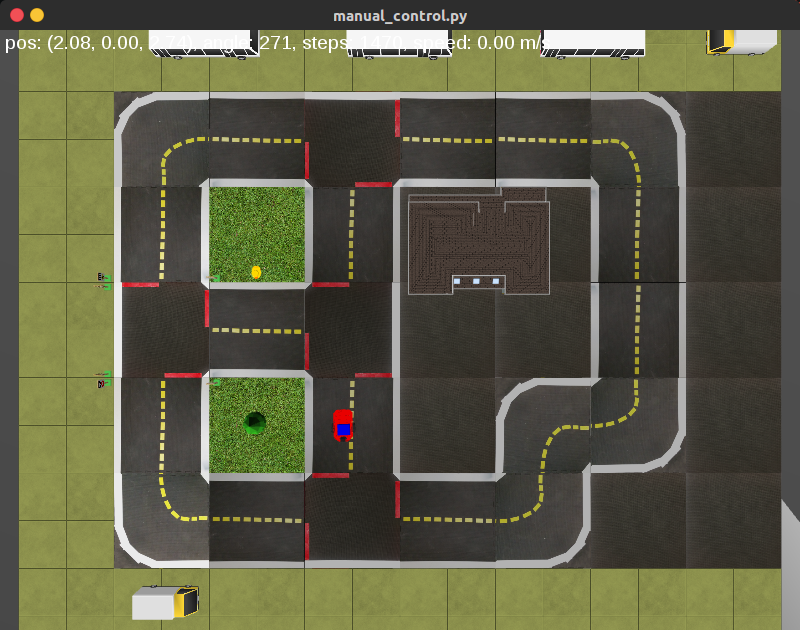
\includegraphics[width=0.6\textwidth]{kapitel2/images/duckietown-umgebung.png}
	\label{fig:duckietown-umgebung}
	\caption{Darstellung einer beispielhaften DuckieTown-Umgebung}
\end{figure}

\section{DuckieBot}

Ein \href{https://get.duckietown.com/products/duckiebot-db18}{DuckieBot} ist ein kleiner mobiler Roboter mit Differenzialantrieb, der seine Umgebung über eine Kamera wahrnehmen kann. Er ist mit einem \href{https://www.raspberrypi.org/}{Raspberry Pi} ausgestattet, welcher für Berechnungen und die Datenverarbeitung zuständig ist. Die  Räder werden über Gleichstrommotoren angetrieben. Mittels eines Steuerbefehls kann ein DuckieBot in einer Umgebung navigiert werden. \cite{duckietown_platform}

\begin{figure}[H]
	\centering
	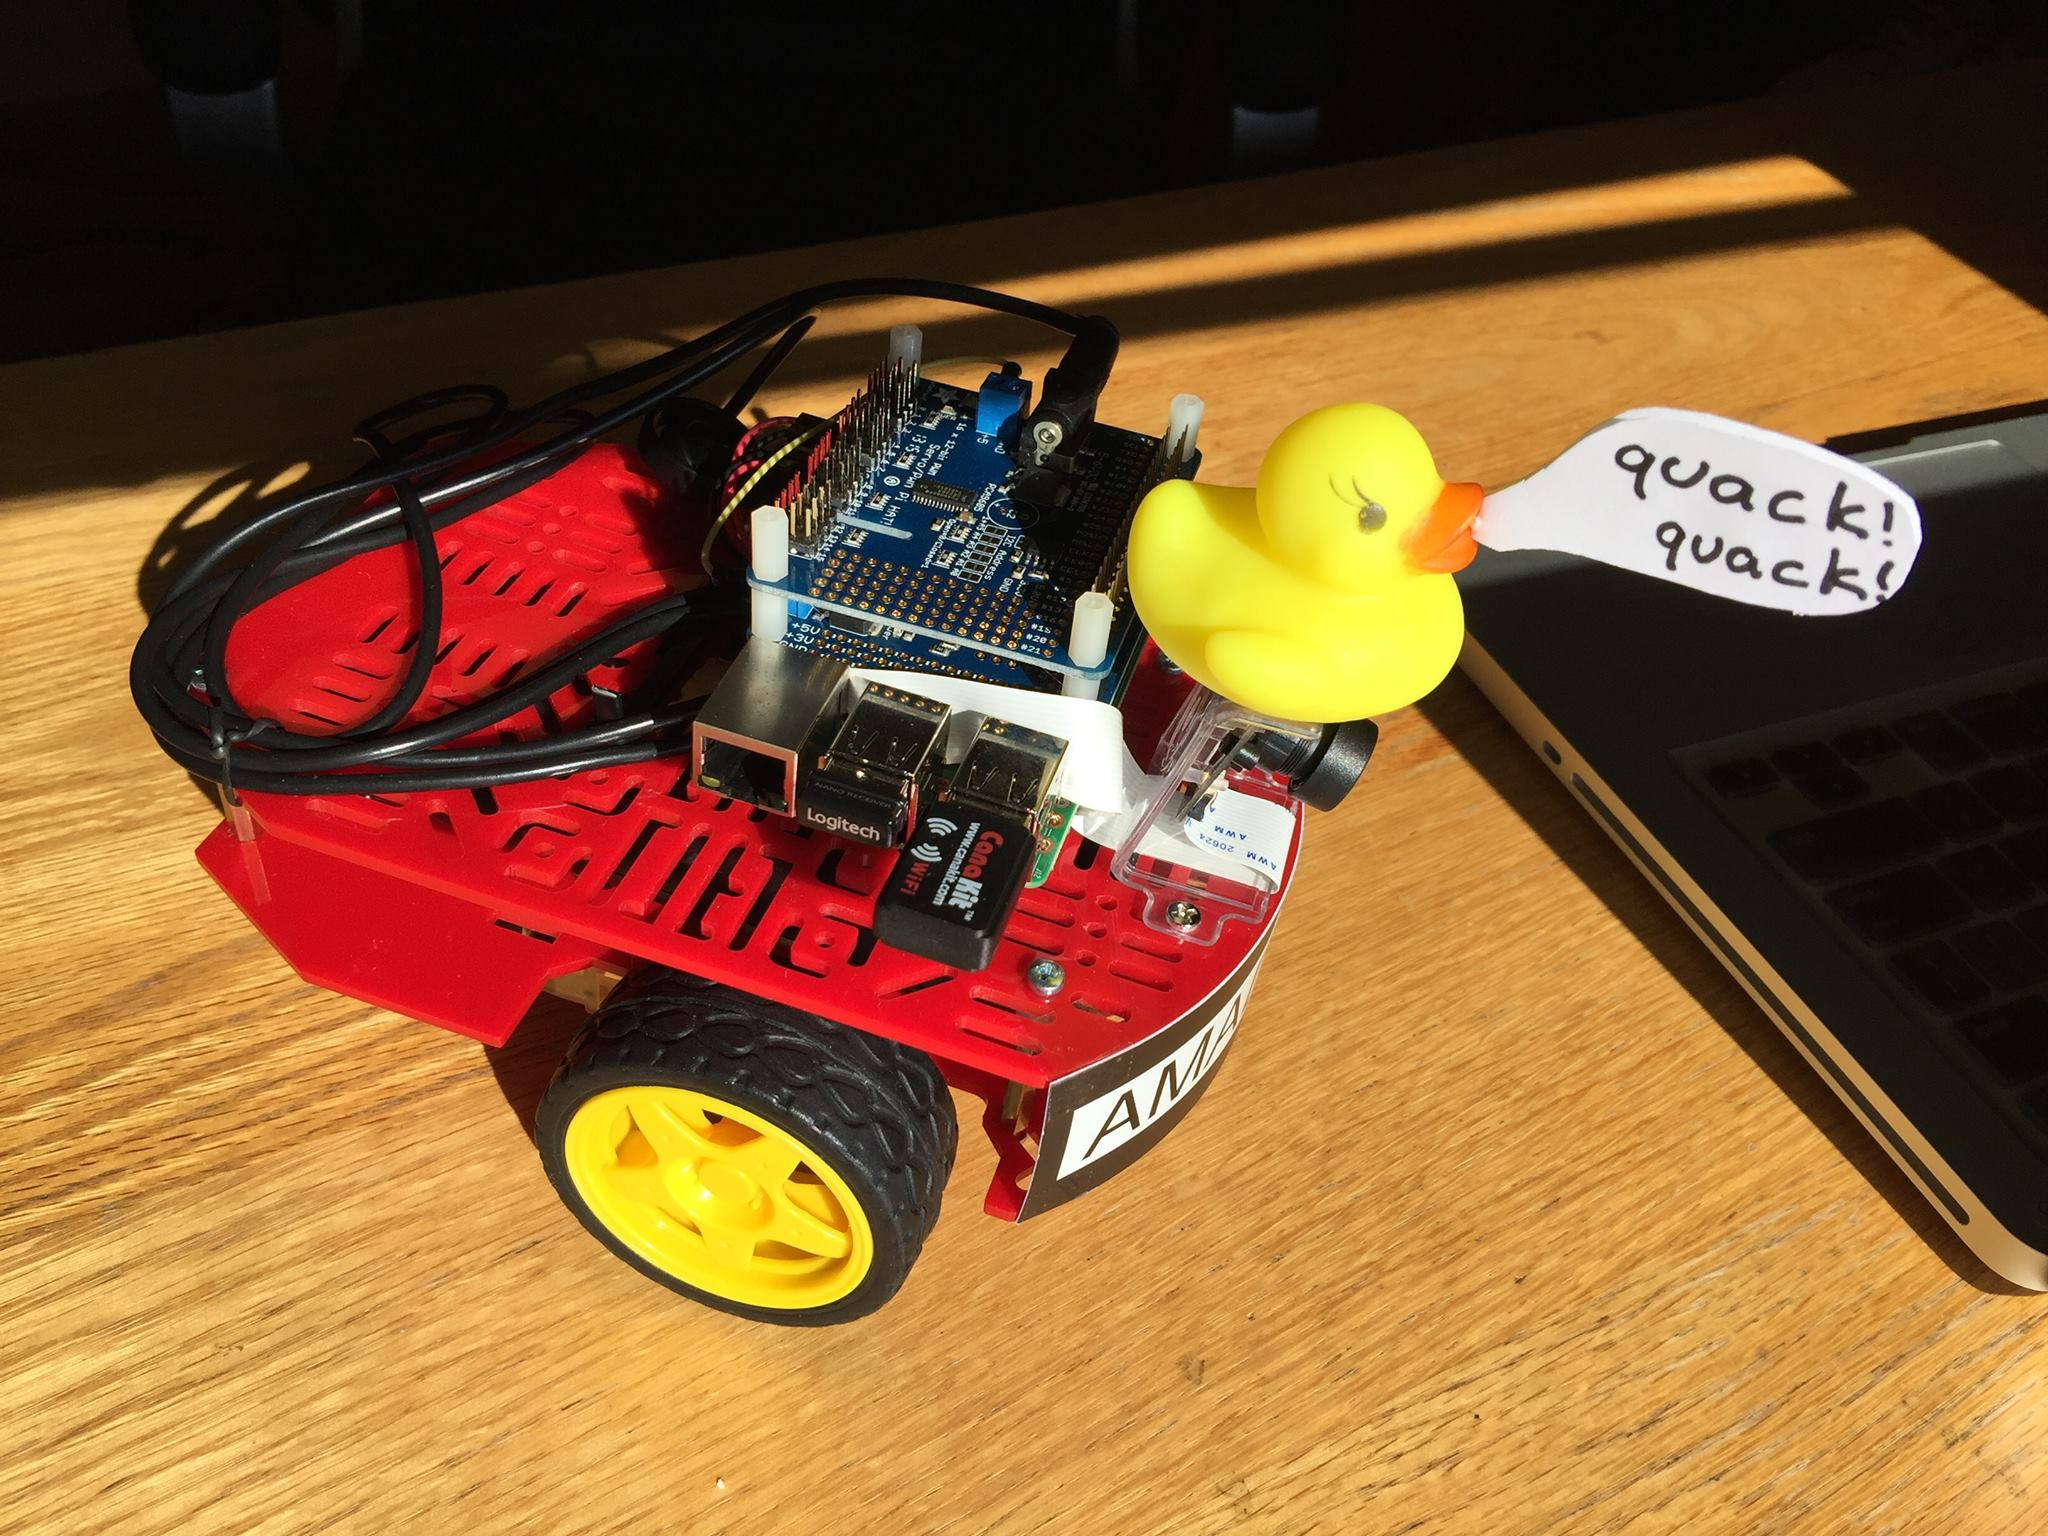
\includegraphics[width=0.5\textwidth]{kapitel2/images/duckiebot.jpg}
	\label{fig:duckiebot}
	\caption{DuckieBot}
\end{figure}


\section{Simulator}

Der \href{https://github.com/duckietown/gym-duckietown}{DuckieTown-Simulator} ist ein in \href{https://www.python.org/}{\texttt{Python}} und \href{https://www.opengl.org/}{\texttt{OpenGL}} \acf{bzw} \href{http://pyglet.org/}{\texttt{Pyglet}} geschriebener Simulator für das \glqq DuckieTown-Universum\grqq. Der Simulator bietet die Möglichkeit DuckieBots (Agenten) in einer beliebigen DuckieTown-Umgebung zu platzieren und die Agenten darin zu navigieren. Eine DuckieTown-Umgebung beinhaltet hierbei eine Menge von befahrbaren Straßenstücken, eine Menge Hindernisse, sowie nicht befahrbare Umgebungsabschnitte. \cite{gym_duckietown} \\

\begin{figure}[H]
	\centering
	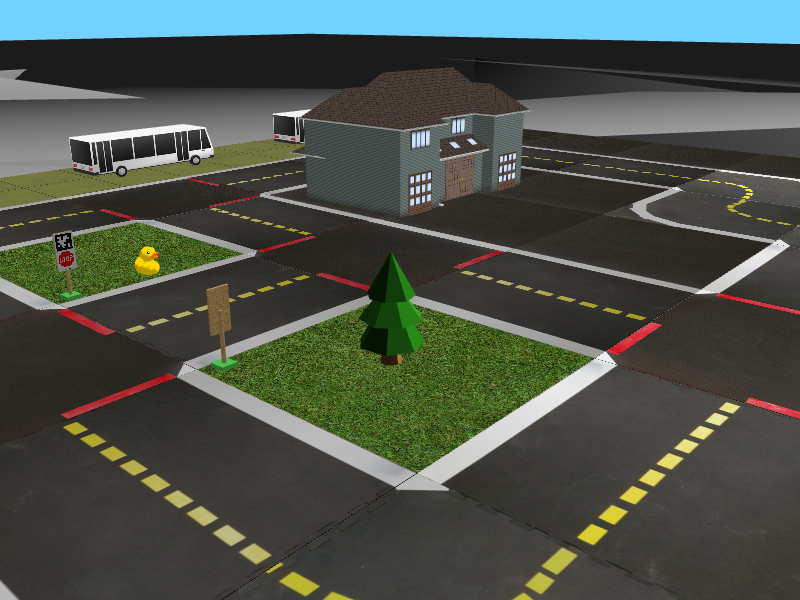
\includegraphics[width=0.6\textwidth]{kapitel2/images/duckietown-gym.png}
	\label{fig:duckietown-gym}
	\caption{DuckieTown-Simulator}
\end{figure}

Der Simulator ist schnell, quelloffen und ausgesprochen anpassungsfähig. Er wurde zunächst für die einfache Linienverfolgung konzipiert und wurde dann im Laufe der Zeit zu einem voll funktionsfähigen Simulator für autonom fahrende Fahrzeuge, insbesondere im Bezug zur künstlichen Intelligenz. \cite{gym_duckietown}



\chapter{Deep Learning}

\section{Was ist Deep Learning?}

Unter \textbf{Deep Learning} (zu deutsch tiefes Lernen) versteht man ein Teilgebiet des maschinellen Lernens, welches sich mit künstlichen neuronalen Netzen und große Datenmengen befasst. Es eignet sich für eine Vielzahl von Anwendungsfällen wie beispielsweiße für selbstfahrende Autos, in der Medizin als auch im Marketing. \cite{datasolut2}\\

Mit Deep Learning können Probleme gelöst werden, die ohne diese Ansätze nicht lösbar wären. Tiefes Lernen ist allerdings sehr rechenaufwändig, wodurch das Training über Monate hinweg andauern kann, um gute Entscheidungen treffen zu können. Gründe hierfür sind komplexe Architekturen sowie eine Vielzahl an Modell-Parametern. \cite{datasolut2} \\

\begin{figure}[H]
	\centering
	\includegraphics[width=\textwidth]{kapitel3/images/KI_Übersicht.png}
	\label{fig:ki-übersicht}
	\caption{Übersicht Künstliche Intelligenz}
\end{figure}

Die Grundlage des Deep Learnings stellt die Verwendung von künstlichen neuronalen Netzen dar. Unter künstlichen neuronalen Netzen versteht man Algorithmen, die nach dem biologischen Vorbild des menschlichen Gehirns modelliert sind. Diese werden eingesetzt, um beispielsweise Muster in Bildern zu erkennen oder Bilder zu klassifizieren. \cite{datasolut2}\\

Ein einfaches künstliches neuronales Netz besteht dabei aus einer \textbf{Eingabeschicht} (Input Layer), einer \textbf{Zwischenschicht} (Hidden Layer) und einer \textbf{Ausgabeschicht} (Output Layer). \cite{datasolut2}

\begin{figure}[H]
	\centering
	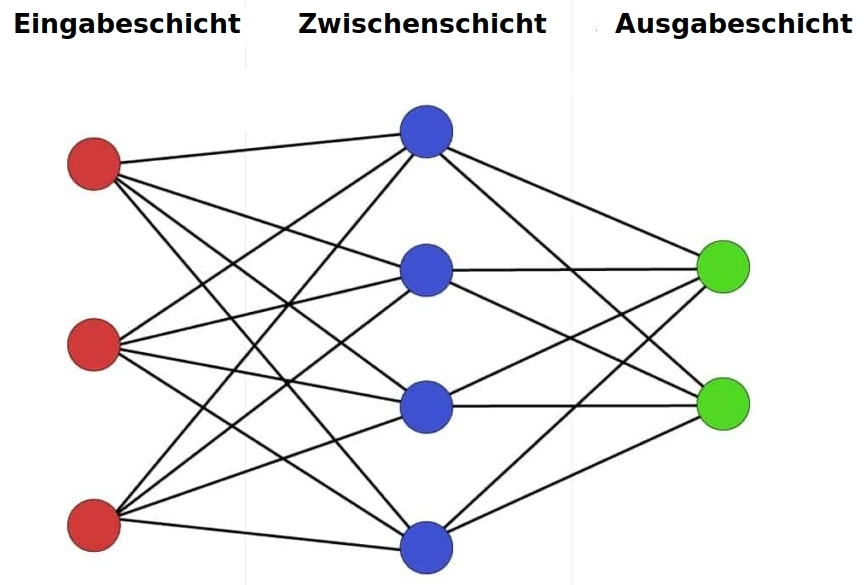
\includegraphics[width=0.65\textwidth]{kapitel3/images/Simples_Neuronales_Netz.jpg}
	\label{fig:simples-neuronales-netz}
	\caption{Darstellung eines beispielhaften künstlichen neuronalen Netzes \\ (vereinfacht)}
\end{figure}

Von tiefem Lernen spricht man dann, wenn die eingesetzen neuronalen Netzte mehr als eine Zwischenschicht haben.  \cite{datasolut2} 

\section{Warum Deep Learning?}

Es gibt Problemstellungen (wie beispielsweise die unstrukturierte Bilderkennung, die sich besonders gut mit künstlichen neuronalen Netzen lösen lassen. Das Erlernen dieser komplexen Muster ist jedoch mit klassischen Machine Leraning Algorithmen nur sehr schwer lösbar. Hier kommen dann tiefe künstliche neuronale Netze zum Einsatz. Je größer die Datenmenge ist, die zum lernen verwendet wird, desto besser funktioniert das tiefe Lernen.

\begin{figure}[H]
	\centering
	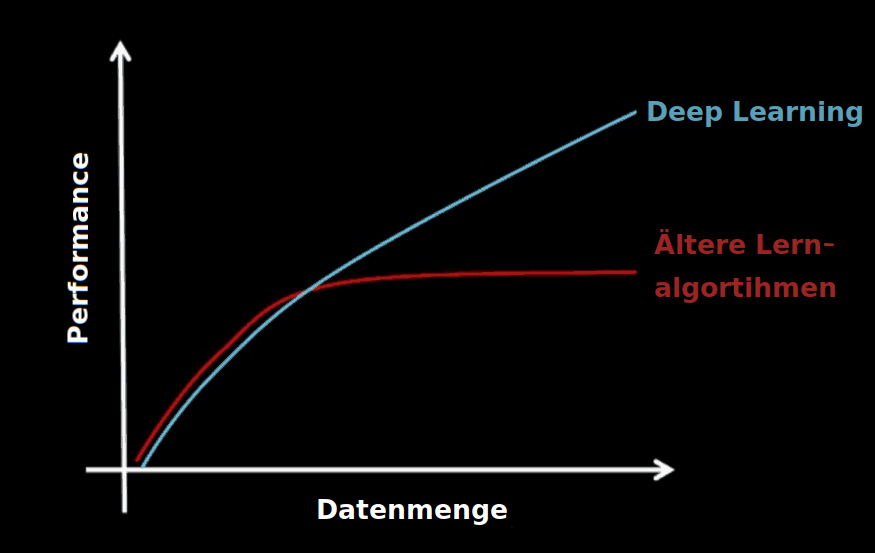
\includegraphics[width=0.65\textwidth]{kapitel3/images/Deep_Learning_Performance.png}
	\label{fig:deep-learning-performance}
	\caption{Darstellung der Performance von Deep Learning Algorithmen im Vergleich zu älteren Lernalgorithmen}
\end{figure}




\section{Problemstellung}

Gegeben sei ein Kamerabild $I_D$, welches von einem Duckiebot $D$ aufgenommen wurde. Das Bild $I_D$ wird einem Posenschätzer $E$ zur Verfügung gestellt, welcher dann den Abstand $d_D$ sowie die Orientierung $\Theta_D$ des Duckiebots zur rechten 
Fahrbahnmarkierung ermitteln soll. Der Posenschätzer ist hierbei ein künstliches neuronales Netz, um die oben genannte Problemstellung lösen zu können. Als Lernverfahren wird überwachtes Lernen eingesetzt.

\section{Datensatzerstellung}

Damit der Posenschätzer seine Aufgabe erfüllen kann, muss zunächst ein Datensatz erstellt werden, damit dieser trainiert werden kann. Der Datensatz besteht dabei aus einem Trainingsdatensatz, einem Validierungsdatensatz sowie aus einem Testdatensatz. \\

Der Trainingsdatensatz ist ein Beispieldatensatz der für das Lernen der Muster und Zusammenhänge in den Daten verwendet wird. Das Modell des neuronalen Netz nutzt also diese Daten um zu lernen. \cite{datasolut} \\

Der Validierungsdatensatz ist ebenso ein Beispieldatensatz, welcher für die Abstimmung der Hyperparameter des Modells des neuronalen Netzes verwendet wird. Dadurch wird das sognenannte \glqq Overfitting\grqq{} (Überanpassung) des Modells auf die Trainingsdaten verhindert. \cite{datasolut} \\

Der Testdatensatz ist ebenfalls ein Beispieldatensatz, jedoch sind die Daten von den Trainingsdaten unabhängig. Die Testdaten werden beim Training des neuronalen Netzes nicht benutzt, sondern dienen zur abschließenden Verifikation des Modells. Dadurch kann die Qualität des Modell erfasst werden, damit man eine Aussage über die Leistungsfähigkeit des neuronalen Netzes treffen kann. \cite{datasolut} \\

Die oben genannten Datensätze wurden mit Hilfe des Duckietownsimulators automatisiert erstellt. Ein Eintrage eines Datensatzes besteht hierbei aus dem Kamerabild $I_D$, welches mit dem dazugehörigen Abstandswert $d_D$ sowie Orientierungswert $\Theta_D$ beschriftet wurde. Der Trainingsdatensatz besteht hierbei aus X Einträgen, der Validierungsdatensatz aus X Einträgen und der Testdatensatz aus X Einträgen. Die Abbildung \ref{fig:data_entry_example} zeigt einige beispielhafte Einträge eines Datensatzes.

\begin{figure}[H]
	\centering
	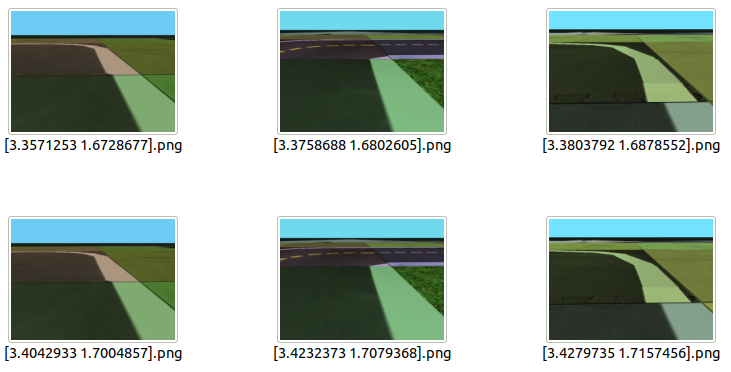
\includegraphics[width=0.8\textwidth]{kapitel3/images/dataset_entries_example.png}
	\caption{Beispielhafte Einträge eines Datensatzes}
	\label{fig:data_entry_example}
\end{figure}


\section{Netzwerkarchitektur}






\chapter{Vorgehensweise}


\chapter{Ergebnisse}


\chapter{Fazit}

\section{Rückblick}

\section{Verbesserungen}

\listoffigures
\bibliographystyle{unsrt}
\bibliography{citeulike} 
\end{document}

